\documentclass{article}
\usepackage[spanish]{babel}
\usepackage[utf8]{inputenc}
\usepackage{amsmath}
\usepackage{graphicx}
\usepackage{hyperref}

\title{Modelo Computacional para Intervalos de Confianza en Precios de Activos Financieros}
\author{Luis Ernesto Amat Cárdenas C-312}
\date{\today}

\begin{document}

\maketitle

\begin{abstract}
\textbf{Español:} Presentamos un modelo computacional que estima intervalos de confianza para precios de activos financieros y commodities mediante un paseo aleatorio pseudo-log-Laplace. La validación mediante back-testing muestra que el modelo mantiene coberturas cercanas al 95\% para horizontes de 5 días en commodities, aunque su precisión disminuye para activos más volátiles como Bitcoin.

\textbf{English:} We present a computational model that estimates confidence intervals for financial assets and commodities prices using a pseudo-log-Laplace random walk. Back-testing validation shows the model maintains ~95\% coverage for 5-day horizons in commodities, though accuracy degrades for more volatile assets like Bitcoin.
\end{abstract}

\section{Estado del Arte}
El modelo clásico para precios de activos \cite{Ross2013} supone:

\begin{equation}
S_n = S_0 \exp\{X_1 + \dots + X_n\}
\end{equation}

donde $X_i \sim \mathcal{N}(\mu,\sigma^2)$. Una generalización común es:

\begin{equation}
S_n = S_0 \prod_{i=1}^n Y_i,\quad Y_i \sim \text{Lognormal}
\end{equation}

Estos modelos fallan al capturar colas pesadas y dependencia serial observadas en mercados reales \cite{Sharpe}.

\section{Modelo Pseudo-log-Laplace}

\subsection{Hipótesis}
Se ha encontrado evidencia a favor de que, para commodities, los rendimientos diarios $X_i$ siguen una distribución de Laplace:

\begin{equation}
f_X(x) = \frac{1}{2b}\exp\left(-\frac{|x-\mu|}{b}\right)
\end{equation}

Validado mediante:
\begin{itemize}
\item Prueba KS ($p > 0.05$ para commodities)
\item Q-Q plots (Figura \ref{fig:qq})
\end{itemize}

También se asume independencia.

Es importante notar que la suma de variables que distribuyen Laplace no distribuye Laplace. Por lo que se deben realizar ajustes a la hora de hacer predicciones analíticas para este modelo.

\begin{figure}[h]
\centering
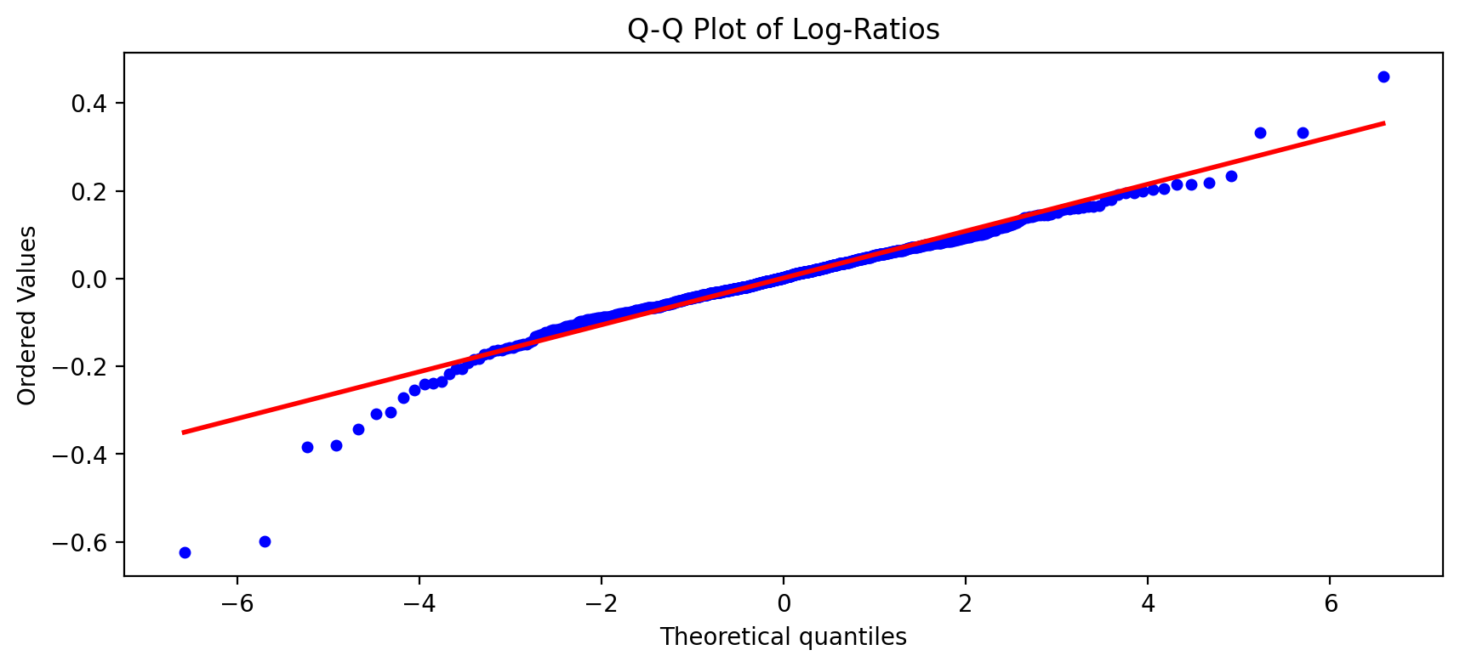
\includegraphics[width=0.6\textwidth]{qq_plot}
\caption{Comparando los datos reales contra la distribución con los parámetros estimados}
\label{fig:qq}
\end{figure}

\subsection{Algoritmo para generar los Intervalos de Confianza (CI)}
\begin{enumerate}
\item Verificar que la variable distribuye (o al menos parece distribuir) Laplace
\item Estimación de parámetros por MLE
\item Simulación de trayectorias
\item Cálculo de intervalos (no paramétrico)
\end{enumerate}

\section{Validación}
Metodología:
\begin{itemize}
\item Para cada día $t$, calcular CI para $t+1:t+5$
\item Contar violaciones (precios fuera del CI)
\item Calcular ratio de cobertura
\end{itemize}

Resultados para $\alpha=0.05$:
\begin{table}[h]
\centering
\begin{tabular}{lcc}
Activo & 3 días & 5 días \\
\hline
Petróleo & 99.0\% & 98.2\% \\
Azúcar & 100\% & 97.7\% \\
BTC & 94.8\% & 89.4\% \\
\end{tabular}
\caption{Cobertura observada de CI}
\end{table}

Los resultados se degradan a partir de 10 días.
Nótese que para $\alpha=0.05$, el resultado $99\%$ significa que el CI calculado no se ajusta lo suficiente al precio. O sea, que es demasiado pesimista.

\section{Conclusión}
El modelo:
\begin{itemize}
\item Proporciona coberturas precisas para commodities
\item Degrada progresivamente con el horizonte temporal
\item Menos potente para activos no-Laplace (e.g. BTC)
\end{itemize}

Aplicaciones:
\begin{itemize}
\item Gestión de riesgo en trading
\item Cálculo de márgenes de seguridad (stop-loss)
\end{itemize}

\begin{thebibliography}{9}
\bibitem{Ross2013} 
Ross, S.M. (2013). \textit{Simulation}. 5th ed. Academic Press.

\bibitem{Sharpe}
\href{https://mathweb.ucsd.edu/~msharpe/stockgrowth.pdf}{Sharpe, M. \textit{LOGNORMAL MODEL FOR STOCK PRICES}. UCSD.}
\end{thebibliography}

\end{document}
